\chapter{Tests de Sensibilité}
Dans cette partie nous cherchons à étudier l'évolution du temps de récupération de tous les minerais de l'environnement en fonction du nombre de robots introduits. \\
Le nombre de minerais dans l'environnement est fixé à 40. Étant donné que certains paramètres rentrant en jeu dans l'évaluation de ce temps sont aléatoires (comme exemples, le temps pour aller à la base pour la version réactive, le temps pour trouver la base la première fois pour la version cognitive ou encore le temps pour trouver un minerai), nous répétons la même expérience avec le même nombre de robots un certain nombre de fois (dix ici) et prenons la moyenne des temps des expériences. Cela nous permet d'avoir des valeurs plus fiables. Ensuite, le programme enregistre ces valeurs dans un fichier. Ainsi pour chaque version, un fichier Excel est produit (\textit{reactif.csv} et \textit{cognitif.csv}). Ce sont ces tableaux Excel que nous exploitons par la suite. 

\begin{figure}[!h]
	\begin{center}
		%taille de l'image en largeur
		%remplacer "width" par "height" pour régler la hauteur
		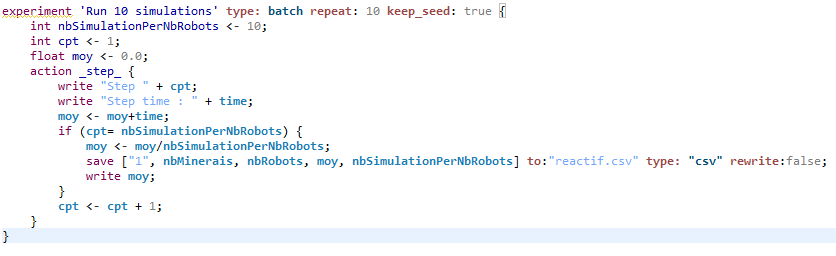
\includegraphics{code/simulations_repetees_reactif}
	\end{center}
	%légende de l'image
	\caption{Simulations répétées de la version réactive}
\end{figure}

\begin{figure}[!h]
	\begin{center}
		%taille de l'image en largeur
		%remplacer "width" par "height" pour régler la hauteur
		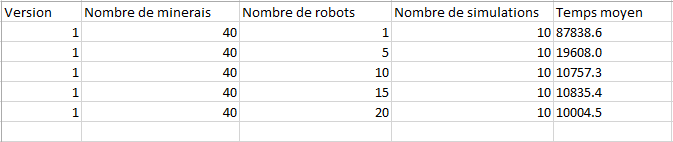
\includegraphics{code/excel_reactif}
	\end{center}
	%légende de l'image
	\caption{Résultat d'exécution des simulations répétées de la version réactive}
\end{figure}

\begin{figure}[!h]
	\begin{center}
		%taille de l'image en largeur
		%remplacer "width" par "height" pour régler la hauteur
		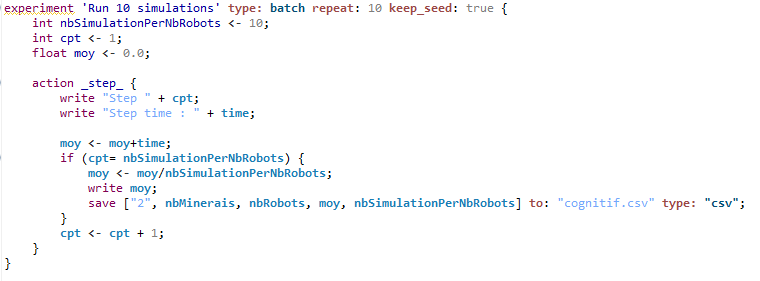
\includegraphics{code/simulations_repetees_cognitif}
	\end{center}
	%légende de l'image
	\caption{Simulations répétées de la version cognitive}
\end{figure}

\begin{figure}[!h]
	\begin{center}
		%taille de l'image en largeur
		%remplacer "width" par "height" pour régler la hauteur
		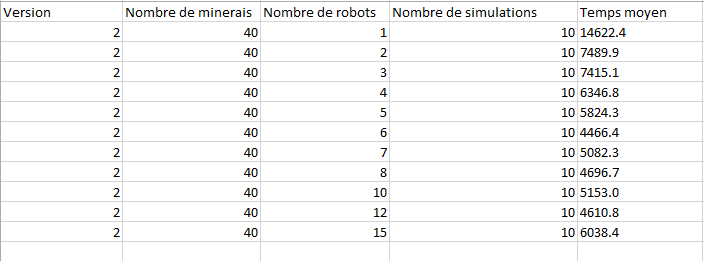
\includegraphics{code/excel_cognitif}
	\end{center}
	%légende de l'image
	\caption{Résultat d'exécution des simulations répétées de la version cognitive}
\end{figure}

\newpage


\section{Robots Réactifs}

%tableau centré à taille variable qui s'ajuste automatiquement suivant la longueur du contenu
\begin{table}[!h]
	\begin{center}
		\begin{tabular}{|r|r|r|r|r|}
			\hline
			Version & Nombre de minerais & Nombre de robots & Nombre de simulations & Temps moyen
			 \\
			\hline
			1 &	40 & 01 & 10 & 87838,6\\
			1 &	40 & 05 & 10 & 19608,0\\
			1 & 40 & 10 & 10 & 10757,3\\
			1 &	40 & 15	& 10 & 10835,4\\
			1 &	40 & 20	& 10 & 10004,5\\
			\hline
		\end{tabular}
	\end{center}
	\caption{Tableau récapitulatif du fichier reactif.csv}
\end{table}
~\\

\begin{center}
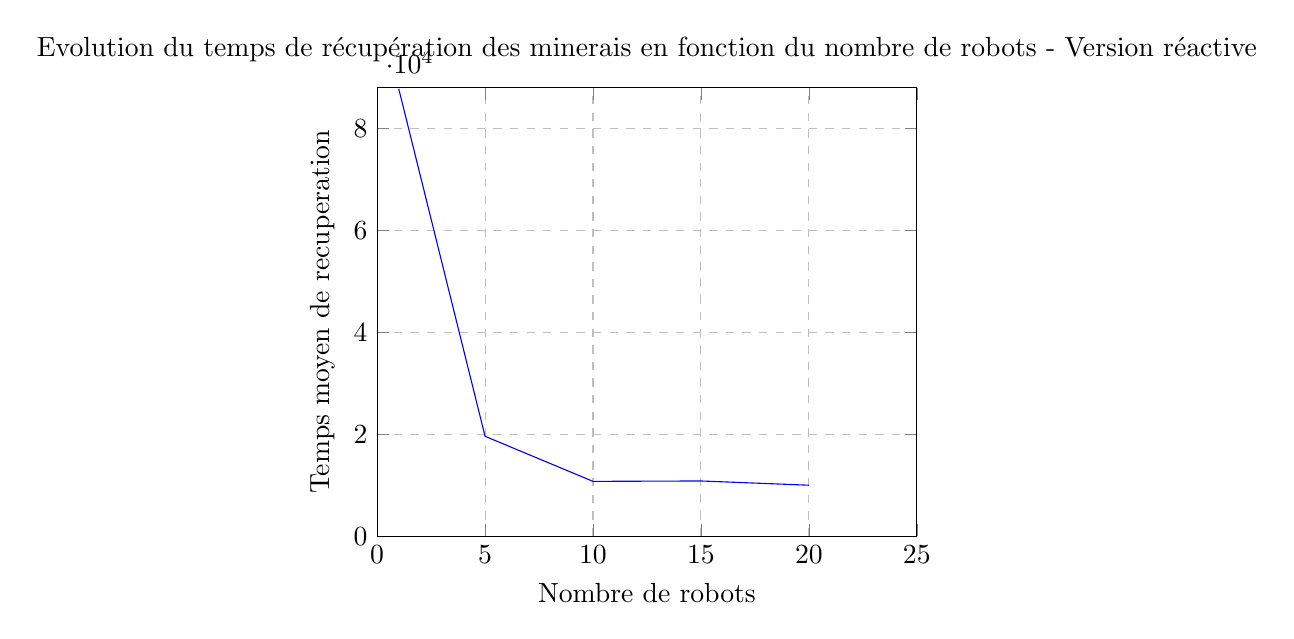
\begin{tikzpicture}
\begin{axis}[
	title = {Evolution du temps de récupération des minerais en fonction du nombre de robots - Version réactive},
	xlabel = {Nombre de robots},
	ylabel = {Temps moyen de recuperation},
	xmin=0, xmax=25,
	ymin=0, ymax=88000,
	xmajorgrids = true,
	ymajorgrids = true,
	grid style = dashed
]

\addplot[
color=blue,
]
coordinates {
	(1,87838.6)(5,19608.0)(10,10757.3)(15,10835.4)(20,10004.5)
};

\end{axis}
\end{tikzpicture}
\end{center}

\paragraph*{Interprétation}
~\\
Nous remarquons que le temps moyen de récupération de tous les minerais diminuent au fur et à mesure que l'on ajoute plus de robots. Cependant, à partir de 10 robots, ce temps devient constant.\\
Concrètement, cela veut dire qu'à partir de 10 robots, il ne sert plus à rien d'augmenter le nombre de robots. Cela ne fait que gaspiller des ressources. \\ Aussi, nous notons que le temps optimal pour les robots réactifs tourne autour de 10000 cycles.

\hskip7mm


\section{Robots Cognitifs}

%tableau centré à taille variable qui s'ajuste automatiquement suivant la longueur du contenu
\begin{table}[!h]
	\begin{center}
		\begin{tabular}{|r|r|r|r|r|}
			\hline
			Version & Nombre de minerais & Nombre de robots & Nombre de simulations & Temps moyen \\
			\hline
			2 &	40 & 01 & 10 & 14622,4\\
			2 &	40 & 02 & 10 &  7489,9\\
			2 & 40 & 03 & 10 &  7415,1\\
			2 &	40 & 04	& 10 &  6346,8\\
			2 &	40 & 05	& 10 &  5824,3\\
			2 &	40 & 06	& 10 &  4466,4\\
			2 &	40 & 07	& 10 &  5082,3\\
			2 &	40 & 08	& 10 &  4696,7\\
			2 &	40 & 10	& 10 &  5153,0\\
			2 &	40 & 12	& 10 &  4610,8\\
			2 &	40 & 15	& 10 &  6038,4\\
			\hline
		\end{tabular}
	\end{center}
	\caption{Tableau récapitulatif du fichier cognitif.csv}
\end{table}


\begin{center}
	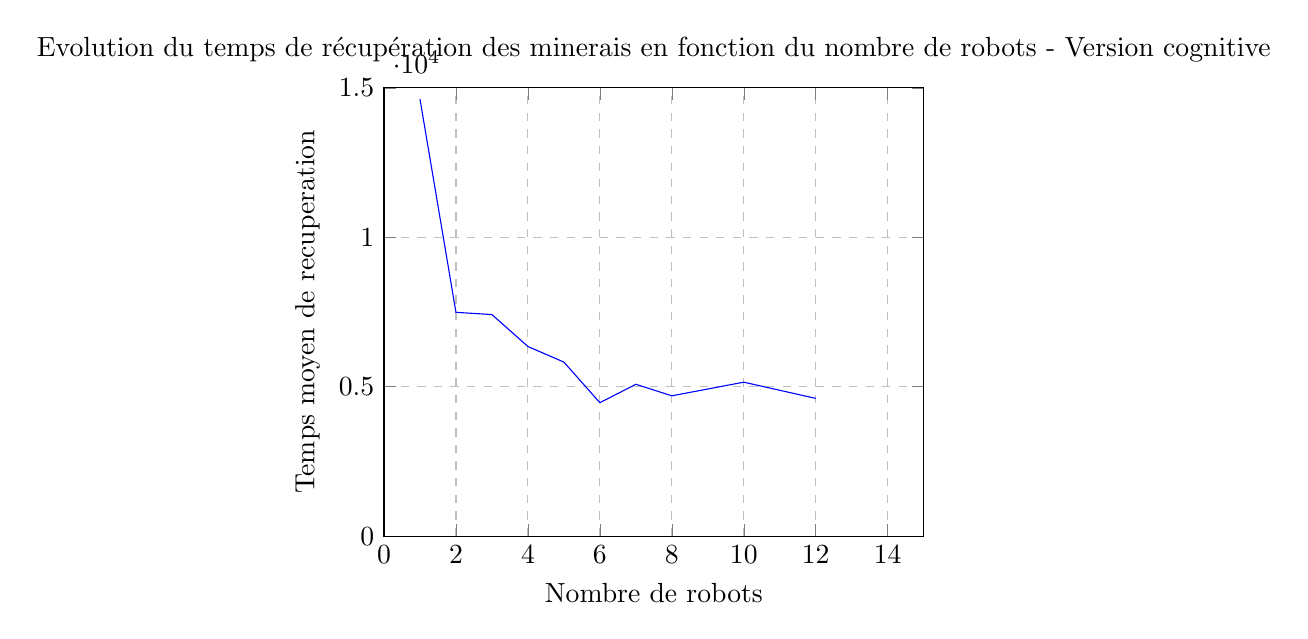
\begin{tikzpicture}
	\begin{axis}[
	title = {Evolution du temps de récupération des minerais en fonction du nombre de robots - Version cognitive},
	xlabel = {Nombre de robots},
	ylabel = {Temps moyen de recuperation},
	xmin=0, xmax=15,
	ymin=0, ymax=15000,
	xmajorgrids = true,
	ymajorgrids = true,
	grid style = dashed
	]
	
	\addplot[
	color=blue,
	]
	coordinates {
		(1,14622.4)(2,7489.9)(3,7415.1)(4,6346.8)(5,5824.3)(6,4466.4)(7,5082.3)(8,4696.7)(10,5153.0)
		(12,4610.8)
	};
	
	\end{axis}
	\end{tikzpicture}
\end{center}

\paragraph*{Interprétation}
~\\
Ici aussi, nous remarquons que le temps moyen de récupération de tous les minerais diminuent au fur et à mesure que l'on ajoute plus de robots. Cependant, ici dès qu'on atteint 6 robots, ce temps devient presque constant.\\
A partir de 6 robots, il n'est plus nécessaire d'ajouter des robots\\ Aussi, nous notons que le temps optimal pour les robots cognitifs tourne autour de 5000 cycles.
\hskip7mm

\section{Version réactive \textit{vs} Version cognitive}

\begin{table}[!h]
	\begin{center}
		\begin{tabular}{|l|r|r|r|}
			\hline
			Version & Nombre de minerais & Nombre de robots & Temps moyen \\
			\hline
			Réactive   & 40 & 01 & 87838,6\\
			Cognitive  & 40 & 01 & 14622,4\\
			\hline
		\end{tabular}
	\end{center}
	\caption{Temps de résolution pour un robot de chaque version}
\end{table}

\begin{align*}
\frac{87838,6}{14622,4} = 6, 0071\\
\end{align*}
Nous remarquons qu'un robot cognitif met approximativement 6 fois moins de temps à récupérer tous les minerais qu'un robot réactif.

\begin{center}
	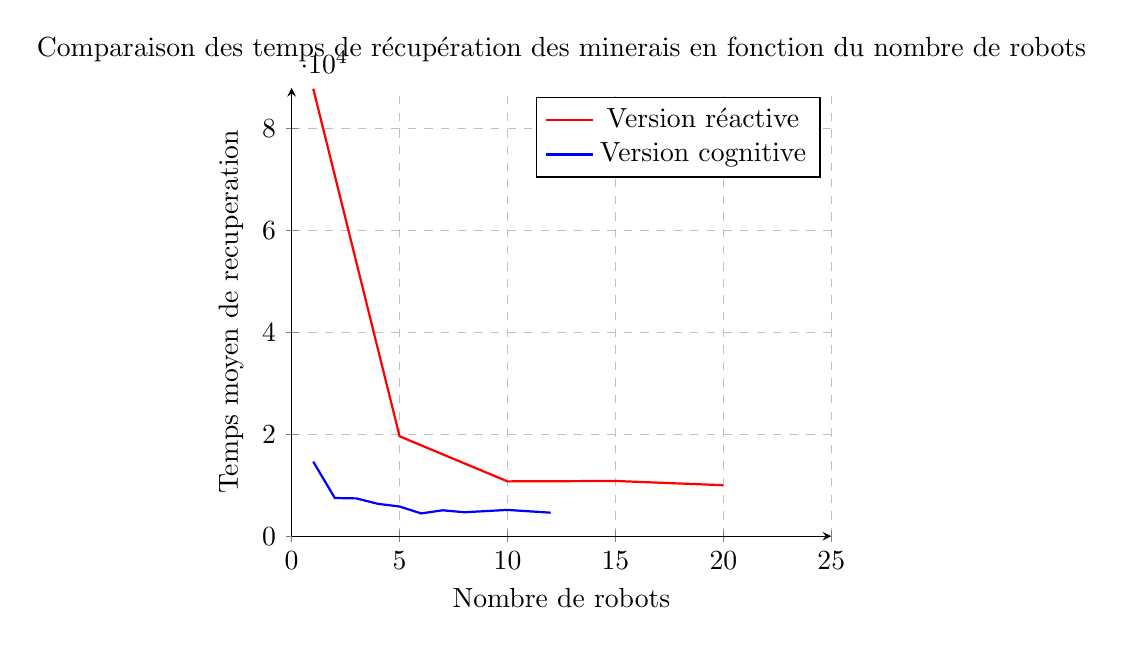
\begin{tikzpicture}
	\begin{axis}[
	title = {Comparaison des temps de récupération des minerais en fonction du nombre de robots},
	xlabel = {Nombre de robots},
	ylabel = {Temps moyen de recuperation},
	xmin=0, xmax=25,
	ymin=0, ymax=88000,
	xmajorgrids = true,
	ymajorgrids = true,
	grid style = dashed,
	axis x line=bottom,
	axis y line=left
	]
	
	\addplot[mark=none,red,thick] coordinates {
		(1,87838.6)(5,19608.0)(10,10757.3)(15,10835.4)(20,10004.5)
	};
	\addlegendentry{Version réactive}
	\addplot[mark=none,blue,thick] coordinates {
		(1,14622.4)(2,7489.9)(3,7415.1)(4,6346.8)(5,5824.3)(6,4466.4)(7,5082.3)(8,4696.7)(10,5153.0)
		(12,4610.8)
	};
	\addlegendentry{Version cognitive}
	\end{axis}
	\end{tikzpicture}
\end{center}
De même, nous remarquons que pour atteindre le temps optimal pour la version réactive, il nous faut introduire jusqu'à 10 robots alors que pour la version cognitive ce temps est atteint à partir de 6 robots. Aussi, à temps optimaux et nombres de robots optimaux, la version cognitive est 2 fois plus rapides (5000 cycles contre 10000 pour la version réactive).\\
Néanmoins, il faut noter que la version cognitive est plus gourmande en ressources alors que la version réactive consomme peu de ressources.\\
Ainsi, nous voyons que chaque version est adapté à une situation bien déterminée. En effet, si on a la possibilité d'avoir plusieurs et que l'on est limité en ressources, il est préférable d'utiliser la version réactive alors que si on est dans une situation ou les ressources ne constituent pas une contrainte, il est plus judicieux d'utiliser la version cognitive qui nous permet d'être plus efficace.